% Set page enumeration
\fancyhf{}
\renewcommand{\headrulewidth}{0pt}
% \lfoot{\textbf{\thepage}}
\pagestyle{fancy}
\fancyfoot[LE,RO]{\textbf{\thepage}}
\setcounter{page}{56}
\setlength{\columnsep}{27pt}

\begin{spacing}{0.8}
\begin{multicols}{2}
\fontdimen2\font=7pt

\noindent треугольника лежит на этой окружности. Найти угол при основании равнобедренного треугольника.

\begin{enumerate}[wide=0pt, labelindent=15pt, label=\textbf{\arabic*}.]
    \setcounter{enumi}{2}
    \itemsep0em
    \item Решить неравенство $3^{\sqrt{x}} > 2^a $.
    \item Решить систему уравнений 
        \[
        \begin{aligned}
            \begin{cases}
                $ \sin{x} + \cos{y} = 0 $, \\
                $ \sin^2{x} + \cos^2{y} = \frac{1}{2}$.
            \end{cases}
        \end{aligned} 
        \]
\end{enumerate}

{\lsstyle Вариант 2}

\begin{enumerate}[wide=0pt, labelindent=15pt, label=\textbf{\arabic*}.]
    \itemsep0em
    \item Сумма первых $n$ членов арифмети-
    ческой прогрессии равна половине суммы
    следующих $n$ членов этой прогрессии. Найти
    отношение суммы первых $3n$ 
    членов прогрессии к сумме ее первых $n$ членов.
    \item В правильную треугольную усечен-
    ную пирамиду с двугранным углом $\alpha$ при основании 
    вписан усеченный конус. Определить
    боковую поверхность конуса, если апофема
    боковой грани пирамиды равна сумме радиусов оснований конуса, а радиус меньшего
    основания конуса равен $r$.
    \item Решить неравенство
    \[
    0,3^{\log_{1/3}{\log_2{\frac{3x+6}{3x^2+2}}}} > 1.
    \]
    \item Решить систему уравнений 
    \[ 
    \begin{aligned}
        \begin{cases}
            $ \sin{x} \cdot \cos{y} = \frac{1}{4} $, \\
            $ 3\tg{x} = \tg{y} $.
        \end{cases}
    \end{aligned} 
    \] 
\end{enumerate}

{\lsstyle Вариант 3}

\begin{enumerate}[wide=0pt, labelindent=15pt, label=\textbf{\arabic*}.]
    \itemsep0em
    \item Если двухзначное число разделить на
произведение его цифр, то в частном полу-
чится 3, а в остатке 9. Если же из квадрата
суммы цифр этого числа вычесть произведе-
ние его цифр, то получится данное число.
Найти это
число.
    \item Куб с ребром а вписан в правильную
    четырехугольную пирамиду так, что четыре
    его вершины находятся на боковых ребрах,
    a четыре другие вершины - на основании
    пирамиды. Боковые грани пирамиды накло-
    нены к плоскости основания под углом $\alpha$.
    Определить объем пирамиды.
    \item Решить уравнение
    \[
    \log_{\sqrt{x}}{a} \cdot \log_{a^2}{\left(\frac{a^2-4}{2a-x}\right)} = 1.
    \]
    \item Решить уравнение
    \[ 
    \cos{\left(x+\frac{\pi}{4}\right)} + \cos{\left(x-\frac{\pi}{4}\right)} = \frac{2}{3}\cos{2x}.
    \]
\end{enumerate}

% \vspace{-11pt}
% \noindent \textbf{Физика}
% \vspace{-26pt} 


\begin{enumerate}[wide=0pt, labelindent=15pt, itemsep=0pt, label=\textbf{\arabic*}.]
    \item Сумма первых $n$ членов арифмети-
    ческой прогрессии равна половине суммы
    следующих $n$ членов этой прогрессии. Найти
    отношение суммы первых $3n$ 
    членов прогрессии к сумме ее первых $n$ членов.
    % \vspace{-6pt}
    \item В однородном
    магнитном поле расположен виток с сопротивлением $R =$ 0,5 \textit{ом}
    и площадью $S = 100$ \textit{см}\textsuperscript{2}. Нормаль к плос-
    кости витка составляет угол $\alpha = 60^{\circ}$ с век-
    тором индукции \textbf{B}. За время $\tau= 0$,5 \textit{сек} ин-
    дукция поля увеличилась с постоянной ско-
    ростью \ от \ $ B_1 =$ 0,1 \textit{тл} \ до \ $B_2=$ 0,6 \textit{тл}. \
    Найти \ количество \ теплоты, \ которое \ выде-
    лилось в витке за это время.
    % \vspace{-6pt}
    \item При облучении
    некоторого металла
    светом сначала с длиной волны $\lambda =$ 0,3 \textit{мкм},
    а затем - с $\lambda =$ 0,6 \textit{мкм} обнаружили, что
    соответствующие
    максимальные скорости
    фотоэлектронов отличаются друг от друга
    в $n=$ 2 раза. Найти работу выхода электро-
    на с поверхности этого металла.
    % \vspace{-40pt}
    \begin{flushright}
        \textit{
        A. Диденко, А. Забоев, \\
        Г. Пантюхов, Н. Шолохов
        }
    \end{flushright}
\end{enumerate}
\end{multicols}

\medskip\hrule\medskip

\noindent {\huge \textbf{Головоломки}} \\ 

{\large \textbf{Магическое домино \hspace*{70pt} 1976}}

\vspace{-21pt}
\setlength{\columnsep}{15pt}
\begin{minipage}{0.29\linewidth}   
    \noindent Из 28 костей домино сложите
    прямоугольник 7x8
    такой,
    что
    если не учитывать семи «пустых» квадратов, образующих последний
    столбец,
    то из 49 к
    клеток
    составлен «магический квадрат» (в котором
    суммируются очки половинок костей) - суммы очков по горизонталям,
    вертикалям и
    двум диагоналям
    одинаковы и равны 24. \\
    \\
    \hspace*{0pt}\hfill \textit{Л. Мочалов}
\end{minipage}
\hspace{3pt}
% \vspace{24pt}
\begin{minipage}{0.64\linewidth}
    \vspace{10pt}
    \begin{multicols}%[2]
        \noindent Расставьте в этих клетках
        числа
        от 1 до 27 (четыре
        числа уже стоят) так, чтобы
        суммы чисел в \columnbreak каждом 
        горизонтальном ряду были
        равны друг другу и суммам
        каждых восьми чисел, стоящих вокруг чисел 1, 9, 7, 6.
    \end{multicols}   
    \hspace{15pt}
    \begin{TAB}(r,2cm,1cm)[14pt]{|c|c|c|c|c|c|c|c|c|}{|c|c|c|}% (rows,min,max)[tabcolsep]{columns}{rows}
        \ & \ & \ & \ & \ & \ & \ & \ & \ &  \\
        \ & 1 & \ & 9 & \ & 7 & \ & 6 & \ &  \\
        \ & \ & \ & \ & \ & \ & \ & \ & \ &  \\
    \end{TAB}
    \vspace{0pt}
    \hspace*{0pt}\hfill \textit{Я. Алексеев}
\end{minipage}


\newpage
\vspace{-10pt}
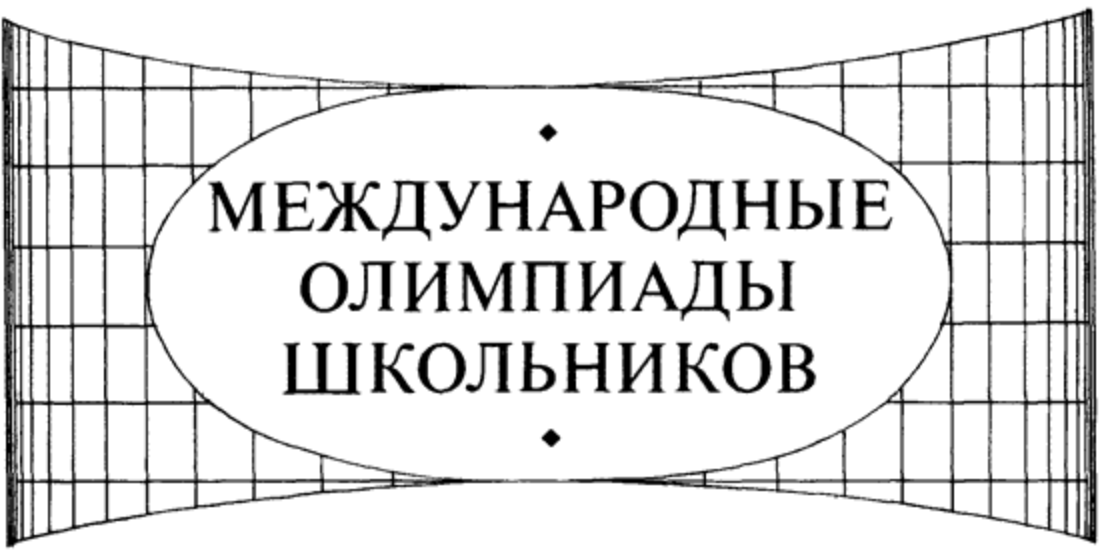
\includegraphics[width=\textwidth, scale=1.2]{images/kvant_math_olymp.png}
% \vspace{19pt}
% \setstretch{25pt}
\setlength{\columnsep}{30pt}
\begin{minipage}{0.47\linewidth}
    \vspace{12pt}
    \textit{3. Моисеева, \\ 
            A. Савин}
    \\[12pt]
    {\Huge \textbf{XVIII Олимпиада по математике}}
    \\[12pt]
    XVIII Международная математическая олимпиада проходила в июле
    1976 г. в г. Лиенце (Австрия). В ней принимали участие коман-
\end{minipage}
\hspace{20pt}
\begin{minipage}{0.47\linewidth}
    \vspace{14pt}
    % \textit{3. Моисеева, \\ 
    %         A. Савин}
    дах этого и прошлых лет, и был определен 
    окончательный состав команды.
    В нее вошли: Юрий Буров (школа
    № 2 г. Москвы), Александр Гончаров
    (школа № 13 г. Никополя Днепропетровской 
    обл.), Петр Гриневич (школа № 204 г. Москвы), 
    Сергей Миронов \ (школа № 6 г. Сафоново Смоленской 
    обл.), Никита Нецветаев, Борис
    Соломяк и Сергей Финашин \ (все --
    ФМШ № 45 \ г. Ленинграда), Татьяна Хованова (школа № 444 г. %Москвы).

\end{minipage}

\end{spacing}
